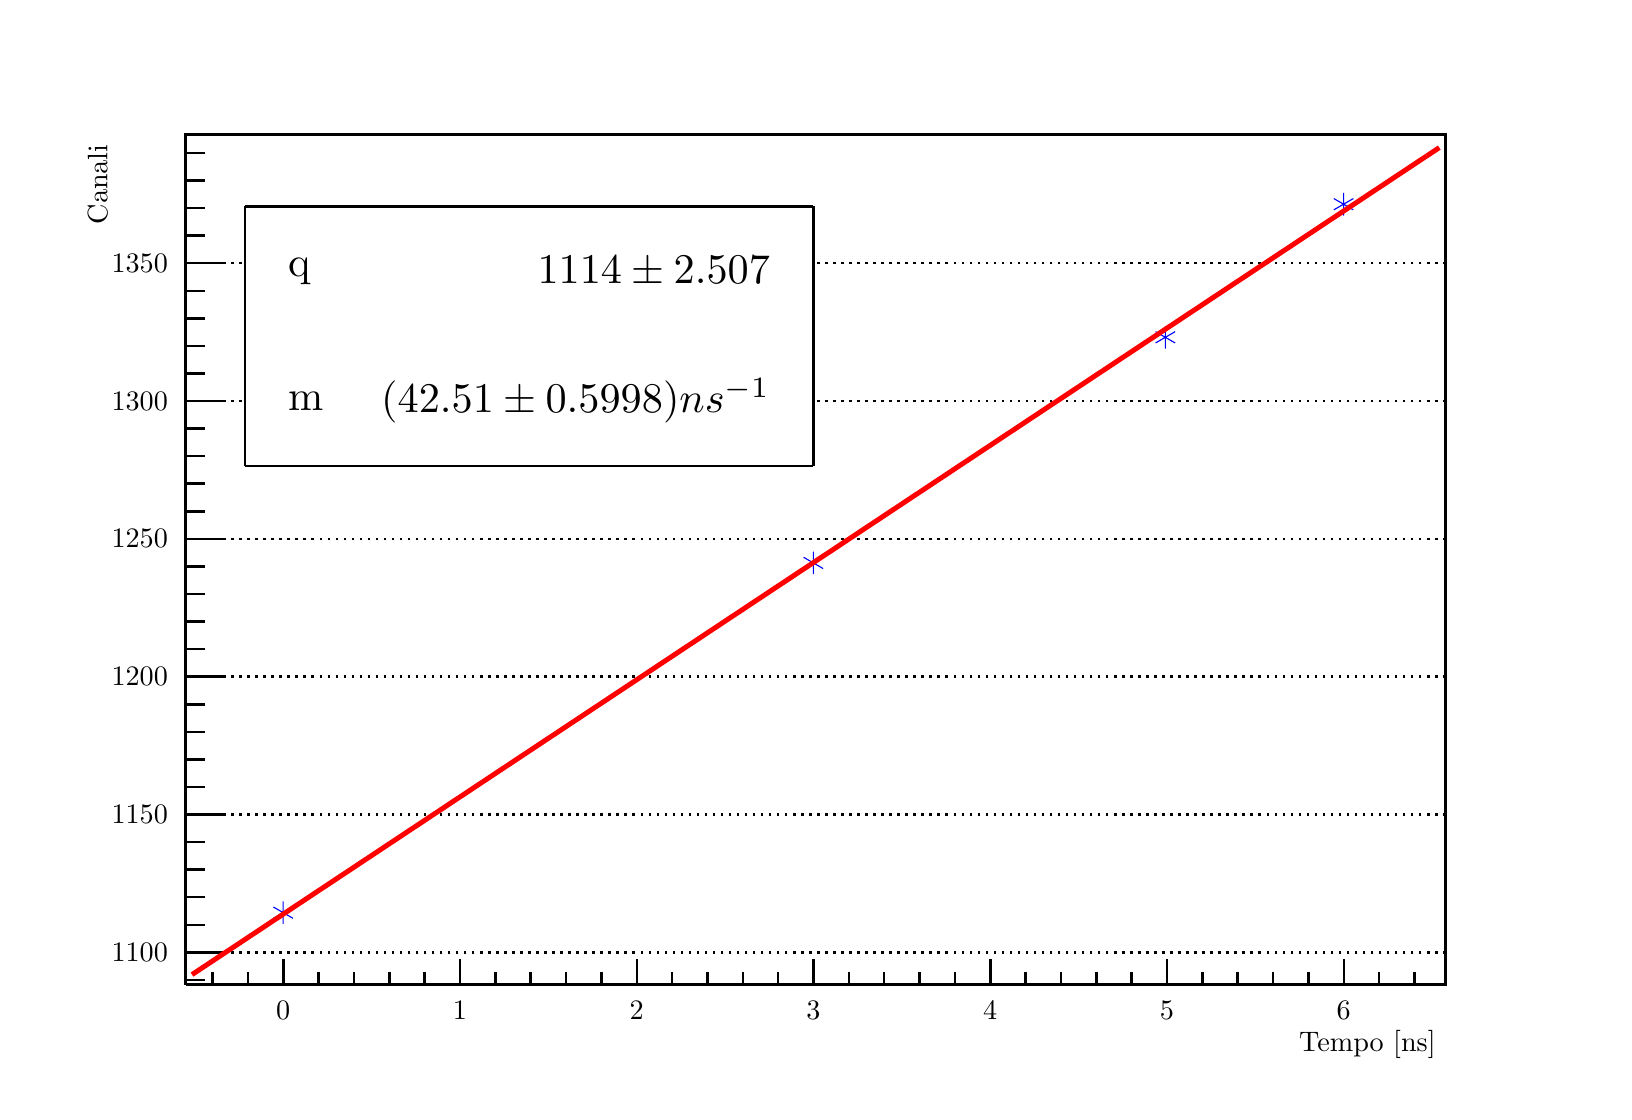
\begin{tikzpicture}
\pgfdeclareplotmark{cross} {
\pgfpathmoveto{\pgfpoint{-0.3\pgfplotmarksize}{\pgfplotmarksize}}
\pgfpathlineto{\pgfpoint{+0.3\pgfplotmarksize}{\pgfplotmarksize}}
\pgfpathlineto{\pgfpoint{+0.3\pgfplotmarksize}{0.3\pgfplotmarksize}}
\pgfpathlineto{\pgfpoint{+1\pgfplotmarksize}{0.3\pgfplotmarksize}}
\pgfpathlineto{\pgfpoint{+1\pgfplotmarksize}{-0.3\pgfplotmarksize}}
\pgfpathlineto{\pgfpoint{+0.3\pgfplotmarksize}{-0.3\pgfplotmarksize}}
\pgfpathlineto{\pgfpoint{+0.3\pgfplotmarksize}{-1.\pgfplotmarksize}}
\pgfpathlineto{\pgfpoint{-0.3\pgfplotmarksize}{-1.\pgfplotmarksize}}
\pgfpathlineto{\pgfpoint{-0.3\pgfplotmarksize}{-0.3\pgfplotmarksize}}
\pgfpathlineto{\pgfpoint{-1.\pgfplotmarksize}{-0.3\pgfplotmarksize}}
\pgfpathlineto{\pgfpoint{-1.\pgfplotmarksize}{0.3\pgfplotmarksize}}
\pgfpathlineto{\pgfpoint{-0.3\pgfplotmarksize}{0.3\pgfplotmarksize}}
\pgfpathclose
\pgfusepathqstroke
}
\pgfdeclareplotmark{cross*} {
\pgfpathmoveto{\pgfpoint{-0.3\pgfplotmarksize}{\pgfplotmarksize}}
\pgfpathlineto{\pgfpoint{+0.3\pgfplotmarksize}{\pgfplotmarksize}}
\pgfpathlineto{\pgfpoint{+0.3\pgfplotmarksize}{0.3\pgfplotmarksize}}
\pgfpathlineto{\pgfpoint{+1\pgfplotmarksize}{0.3\pgfplotmarksize}}
\pgfpathlineto{\pgfpoint{+1\pgfplotmarksize}{-0.3\pgfplotmarksize}}
\pgfpathlineto{\pgfpoint{+0.3\pgfplotmarksize}{-0.3\pgfplotmarksize}}
\pgfpathlineto{\pgfpoint{+0.3\pgfplotmarksize}{-1.\pgfplotmarksize}}
\pgfpathlineto{\pgfpoint{-0.3\pgfplotmarksize}{-1.\pgfplotmarksize}}
\pgfpathlineto{\pgfpoint{-0.3\pgfplotmarksize}{-0.3\pgfplotmarksize}}
\pgfpathlineto{\pgfpoint{-1.\pgfplotmarksize}{-0.3\pgfplotmarksize}}
\pgfpathlineto{\pgfpoint{-1.\pgfplotmarksize}{0.3\pgfplotmarksize}}
\pgfpathlineto{\pgfpoint{-0.3\pgfplotmarksize}{0.3\pgfplotmarksize}}
\pgfpathclose
\pgfusepathqfillstroke
}
\pgfdeclareplotmark{newstar} {
\pgfpathmoveto{\pgfqpoint{0pt}{\pgfplotmarksize}}
\pgfpathlineto{\pgfqpointpolar{44}{0.5\pgfplotmarksize}}
\pgfpathlineto{\pgfqpointpolar{18}{\pgfplotmarksize}}
\pgfpathlineto{\pgfqpointpolar{-20}{0.5\pgfplotmarksize}}
\pgfpathlineto{\pgfqpointpolar{-54}{\pgfplotmarksize}}
\pgfpathlineto{\pgfqpointpolar{-90}{0.5\pgfplotmarksize}}
\pgfpathlineto{\pgfqpointpolar{234}{\pgfplotmarksize}}
\pgfpathlineto{\pgfqpointpolar{198}{0.5\pgfplotmarksize}}
\pgfpathlineto{\pgfqpointpolar{162}{\pgfplotmarksize}}
\pgfpathlineto{\pgfqpointpolar{134}{0.5\pgfplotmarksize}}
\pgfpathclose
\pgfusepathqstroke
}
\pgfdeclareplotmark{newstar*} {
\pgfpathmoveto{\pgfqpoint{0pt}{\pgfplotmarksize}}
\pgfpathlineto{\pgfqpointpolar{44}{0.5\pgfplotmarksize}}
\pgfpathlineto{\pgfqpointpolar{18}{\pgfplotmarksize}}
\pgfpathlineto{\pgfqpointpolar{-20}{0.5\pgfplotmarksize}}
\pgfpathlineto{\pgfqpointpolar{-54}{\pgfplotmarksize}}
\pgfpathlineto{\pgfqpointpolar{-90}{0.5\pgfplotmarksize}}
\pgfpathlineto{\pgfqpointpolar{234}{\pgfplotmarksize}}
\pgfpathlineto{\pgfqpointpolar{198}{0.5\pgfplotmarksize}}
\pgfpathlineto{\pgfqpointpolar{162}{\pgfplotmarksize}}
\pgfpathlineto{\pgfqpointpolar{134}{0.5\pgfplotmarksize}}
\pgfpathclose
\pgfusepathqfillstroke
}
\definecolor{c}{rgb}{1,1,1};
\draw [color=c, fill=c] (0,0) rectangle (20,13.4957);
\draw [color=c, fill=c] (2,1.34957) rectangle (18,12.1461);
\definecolor{c}{rgb}{0,0,0};
\draw [c,line width=0.9] (2,1.34957) -- (2,12.1461) -- (18,12.1461) -- (18,1.34957) -- (2,1.34957);
\definecolor{c}{rgb}{1,1,1};
\draw [color=c, fill=c] (2,1.34957) rectangle (18,12.1461);
\definecolor{c}{rgb}{0,0,0};
\draw [c,line width=0.9] (2,1.34957) -- (2,12.1461) -- (18,12.1461) -- (18,1.34957) -- (2,1.34957);
\draw [c,line width=0.9] (2,1.34957) -- (18,1.34957);
\draw [c,line width=0.9] (2,1.34957) -- (2,12.1461);
\draw [c,dotted,line width=0.9] (18,1.75917) -- (2,1.75917);
\draw [c,dotted,line width=0.9] (18,3.50958) -- (2,3.50958);
\draw [c,dotted,line width=0.9] (18,5.26) -- (2,5.26);
\draw [c,dotted,line width=0.9] (18,7.01041) -- (2,7.01041);
\draw [c,dotted,line width=0.9] (18,8.76083) -- (2,8.76083);
\draw [c,dotted,line width=0.9] (18,10.5112) -- (2,10.5112);
\draw [c,dotted,line width=0.9] (18,1.75917) -- (2,1.75917);
\draw [c,dotted,line width=0.9] (18,10.5112) -- (2,10.5112);
\draw [c,line width=0.9] (2,1.34957) -- (18,1.34957);
\draw [anchor= east] (18,0.593811) node[scale=1.01821, color=c, rotate=0]{Tempo [ns]};
\draw [c,line width=0.9] (3.23906,1.67347) -- (3.23906,1.34957);
\draw [c,line width=0.9] (3.68799,1.51152) -- (3.68799,1.34957);
\draw [c,line width=0.9] (4.13692,1.51152) -- (4.13692,1.34957);
\draw [c,line width=0.9] (4.58586,1.51152) -- (4.58586,1.34957);
\draw [c,line width=0.9] (5.03479,1.51152) -- (5.03479,1.34957);
\draw [c,line width=0.9] (5.48373,1.67347) -- (5.48373,1.34957);
\draw [c,line width=0.9] (5.93266,1.51152) -- (5.93266,1.34957);
\draw [c,line width=0.9] (6.38159,1.51152) -- (6.38159,1.34957);
\draw [c,line width=0.9] (6.83053,1.51152) -- (6.83053,1.34957);
\draw [c,line width=0.9] (7.27946,1.51152) -- (7.27946,1.34957);
\draw [c,line width=0.9] (7.72839,1.67347) -- (7.72839,1.34957);
\draw [c,line width=0.9] (8.17733,1.51152) -- (8.17733,1.34957);
\draw [c,line width=0.9] (8.62626,1.51152) -- (8.62626,1.34957);
\draw [c,line width=0.9] (9.0752,1.51152) -- (9.0752,1.34957);
\draw [c,line width=0.9] (9.52413,1.51152) -- (9.52413,1.34957);
\draw [c,line width=0.9] (9.97306,1.67347) -- (9.97306,1.34957);
\draw [c,line width=0.9] (10.422,1.51152) -- (10.422,1.34957);
\draw [c,line width=0.9] (10.8709,1.51152) -- (10.8709,1.34957);
\draw [c,line width=0.9] (11.3199,1.51152) -- (11.3199,1.34957);
\draw [c,line width=0.9] (11.7688,1.51152) -- (11.7688,1.34957);
\draw [c,line width=0.9] (12.2177,1.67347) -- (12.2177,1.34957);
\draw [c,line width=0.9] (12.6667,1.51152) -- (12.6667,1.34957);
\draw [c,line width=0.9] (13.1156,1.51152) -- (13.1156,1.34957);
\draw [c,line width=0.9] (13.5645,1.51152) -- (13.5645,1.34957);
\draw [c,line width=0.9] (14.0135,1.51152) -- (14.0135,1.34957);
\draw [c,line width=0.9] (14.4624,1.67347) -- (14.4624,1.34957);
\draw [c,line width=0.9] (14.9113,1.51152) -- (14.9113,1.34957);
\draw [c,line width=0.9] (15.3603,1.51152) -- (15.3603,1.34957);
\draw [c,line width=0.9] (15.8092,1.51152) -- (15.8092,1.34957);
\draw [c,line width=0.9] (16.2581,1.51152) -- (16.2581,1.34957);
\draw [c,line width=0.9] (16.7071,1.67347) -- (16.7071,1.34957);
\draw [c,line width=0.9] (3.23906,1.67347) -- (3.23906,1.34957);
\draw [c,line width=0.9] (2.79012,1.51152) -- (2.79012,1.34957);
\draw [c,line width=0.9] (2.34119,1.51152) -- (2.34119,1.34957);
\draw [c,line width=0.9] (16.7071,1.67347) -- (16.7071,1.34957);
\draw [c,line width=0.9] (17.156,1.51152) -- (17.156,1.34957);
\draw [c,line width=0.9] (17.6049,1.51152) -- (17.6049,1.34957);
\draw [anchor=base] (3.23906,0.904212) node[scale=1.01821, color=c, rotate=0]{0};
\draw [anchor=base] (5.48373,0.904212) node[scale=1.01821, color=c, rotate=0]{1};
\draw [anchor=base] (7.72839,0.904212) node[scale=1.01821, color=c, rotate=0]{2};
\draw [anchor=base] (9.97306,0.904212) node[scale=1.01821, color=c, rotate=0]{3};
\draw [anchor=base] (12.2177,0.904212) node[scale=1.01821, color=c, rotate=0]{4};
\draw [anchor=base] (14.4624,0.904212) node[scale=1.01821, color=c, rotate=0]{5};
\draw [anchor=base] (16.7071,0.904212) node[scale=1.01821, color=c, rotate=0]{6};
\draw [c,line width=0.9] (2,1.34957) -- (2,12.1461);
\draw [anchor= east] (0.88,12.1461) node[scale=1.01821, color=c, rotate=90]{Canali};
\draw [c,line width=0.9] (2.48,1.75917) -- (2,1.75917);
\draw [c,line width=0.9] (2.24,2.10925) -- (2,2.10925);
\draw [c,line width=0.9] (2.24,2.45933) -- (2,2.45933);
\draw [c,line width=0.9] (2.24,2.80942) -- (2,2.80942);
\draw [c,line width=0.9] (2.24,3.1595) -- (2,3.1595);
\draw [c,line width=0.9] (2.48,3.50958) -- (2,3.50958);
\draw [c,line width=0.9] (2.24,3.85967) -- (2,3.85967);
\draw [c,line width=0.9] (2.24,4.20975) -- (2,4.20975);
\draw [c,line width=0.9] (2.24,4.55983) -- (2,4.55983);
\draw [c,line width=0.9] (2.24,4.90991) -- (2,4.90991);
\draw [c,line width=0.9] (2.48,5.26) -- (2,5.26);
\draw [c,line width=0.9] (2.24,5.61008) -- (2,5.61008);
\draw [c,line width=0.9] (2.24,5.96016) -- (2,5.96016);
\draw [c,line width=0.9] (2.24,6.31025) -- (2,6.31025);
\draw [c,line width=0.9] (2.24,6.66033) -- (2,6.66033);
\draw [c,line width=0.9] (2.48,7.01041) -- (2,7.01041);
\draw [c,line width=0.9] (2.24,7.3605) -- (2,7.3605);
\draw [c,line width=0.9] (2.24,7.71058) -- (2,7.71058);
\draw [c,line width=0.9] (2.24,8.06066) -- (2,8.06066);
\draw [c,line width=0.9] (2.24,8.41075) -- (2,8.41075);
\draw [c,line width=0.9] (2.48,8.76083) -- (2,8.76083);
\draw [c,line width=0.9] (2.24,9.11091) -- (2,9.11091);
\draw [c,line width=0.9] (2.24,9.46099) -- (2,9.46099);
\draw [c,line width=0.9] (2.24,9.81108) -- (2,9.81108);
\draw [c,line width=0.9] (2.24,10.1612) -- (2,10.1612);
\draw [c,line width=0.9] (2.48,10.5112) -- (2,10.5112);
\draw [c,line width=0.9] (2.48,1.75917) -- (2,1.75917);
\draw [c,line width=0.9] (2.24,1.40908) -- (2,1.40908);
\draw [c,line width=0.9] (2.48,10.5112) -- (2,10.5112);
\draw [c,line width=0.9] (2.24,10.8613) -- (2,10.8613);
\draw [c,line width=0.9] (2.24,11.2114) -- (2,11.2114);
\draw [c,line width=0.9] (2.24,11.5615) -- (2,11.5615);
\draw [c,line width=0.9] (2.24,11.9116) -- (2,11.9116);
\draw [anchor= east] (1.9,1.75917) node[scale=1.01821, color=c, rotate=0]{1100};
\draw [anchor= east] (1.9,3.50958) node[scale=1.01821, color=c, rotate=0]{1150};
\draw [anchor= east] (1.9,5.26) node[scale=1.01821, color=c, rotate=0]{1200};
\draw [anchor= east] (1.9,7.01041) node[scale=1.01821, color=c, rotate=0]{1250};
\draw [anchor= east] (1.9,8.76083) node[scale=1.01821, color=c, rotate=0]{1300};
\draw [anchor= east] (1.9,10.5112) node[scale=1.01821, color=c, rotate=0]{1350};
\definecolor{c}{rgb}{1,1,1};
\draw [color=c, fill=c] (2.75072,7.93696) rectangle (9.97135,11.2321);
\definecolor{c}{rgb}{0,0,0};
\draw [c,line width=0.9] (2.75072,7.93696) -- (9.97135,7.93696);
\draw [c,line width=0.9] (9.97135,7.93696) -- (9.97135,11.2321);
\draw [c,line width=0.9] (9.97135,11.2321) -- (2.75072,11.2321);
\draw [c,line width=0.9] (2.75072,11.2321) -- (2.75072,7.93696);
\draw [anchor= west] (3.11175,10.4083) node[scale=1.52731, color=c, rotate=0]{q       };
\draw [anchor= east] (9.61032,10.4083) node[scale=1.52731, color=c, rotate=0]{$  1114 \pm 2.507$};
\draw [anchor= west] (3.11175,8.76075) node[scale=1.52731, color=c, rotate=0]{m       };
\draw [anchor= east] (9.61032,8.76075) node[scale=1.52731, color=c, rotate=0]{$ 42.51 \pm 0.5998$};
\definecolor{c}{rgb}{0,0,1};
\foreach \P in {(3.23782,2.26361),(9.97135,6.70487),(14.4413,9.5702),(16.7049,11.2607)}{\draw[mark options={color=c,fill=c},mark size=4.084084pt,mark=asterisk] plot coordinates {\P};}
\definecolor{c}{rgb}{1,0,0};
\draw [c,line width=1.8] (2.08,1.47669) -- (2.24,1.58277) -- (2.4,1.68886) -- (2.56,1.79494) -- (2.72,1.90103) -- (2.88,2.00711) -- (3.04,2.1132) -- (3.2,2.21929) -- (3.36,2.32537) -- (3.52,2.43146) -- (3.68,2.53754) -- (3.84,2.64363) -- (4,2.74971)
 -- (4.16,2.8558) -- (4.32,2.96189) -- (4.48,3.06797) -- (4.64,3.17406) -- (4.8,3.28014) -- (4.96,3.38623) -- (5.12,3.49231) -- (5.28,3.5984) -- (5.44,3.70448) -- (5.6,3.81057) -- (5.76,3.91666) -- (5.92,4.02274) -- (6.08,4.12883) -- (6.24,4.23491)
 -- (6.4,4.341) -- (6.56,4.44708) -- (6.72,4.55317) -- (6.88,4.65926) -- (7.04,4.76534) -- (7.2,4.87143) -- (7.36,4.97751) -- (7.52,5.0836) -- (7.68,5.18968) -- (7.84,5.29577) -- (8,5.40186) -- (8.16,5.50794) -- (8.32,5.61403) -- (8.48,5.72011) --
 (8.64,5.8262) -- (8.8,5.93228) -- (8.96,6.03837) -- (9.12,6.14446) -- (9.28,6.25054) -- (9.44,6.35663) -- (9.6,6.46271) -- (9.76,6.5688) -- (9.92,6.67488);
\draw [c,line width=1.8] (9.92,6.67488) -- (10.08,6.78097) -- (10.24,6.88706) -- (10.4,6.99314) -- (10.56,7.09923) -- (10.72,7.20531) -- (10.88,7.3114) -- (11.04,7.41748) -- (11.2,7.52357) -- (11.36,7.62965) -- (11.52,7.73574) -- (11.68,7.84183) --
 (11.84,7.94791) -- (12,8.054) -- (12.16,8.16008) -- (12.32,8.26617) -- (12.48,8.37226) -- (12.64,8.47834) -- (12.8,8.58443) -- (12.96,8.69051) -- (13.12,8.7966) -- (13.28,8.90268) -- (13.44,9.00877) -- (13.6,9.11485) -- (13.76,9.22094) --
 (13.92,9.32703) -- (14.08,9.43311) -- (14.24,9.5392) -- (14.4,9.64528) -- (14.56,9.75137) -- (14.72,9.85745) -- (14.88,9.96354) -- (15.04,10.0696) -- (15.2,10.1757) -- (15.36,10.2818) -- (15.52,10.3879) -- (15.68,10.494) -- (15.84,10.6001) --
 (16,10.7061) -- (16.16,10.8122) -- (16.32,10.9183) -- (16.48,11.0244) -- (16.64,11.1305) -- (16.8,11.2366) -- (16.96,11.3427) -- (17.12,11.4487) -- (17.28,11.5548) -- (17.44,11.6609) -- (17.6,11.767) -- (17.76,11.8731);
\draw [c,line width=1.8] (17.76,11.8731) -- (17.92,11.9792);
\definecolor{c}{rgb}{1,1,1};
\draw [color=c, fill=c] (2.75072,7.93696) rectangle (9.97135,11.2321);
\definecolor{c}{rgb}{0,0,0};
\draw [c,line width=0.9] (2.75072,7.93696) -- (9.97135,7.93696);
\draw [c,line width=0.9] (9.97135,7.93696) -- (9.97135,11.2321);
\draw [c,line width=0.9] (9.97135,11.2321) -- (2.75072,11.2321);
\draw [c,line width=0.9] (2.75072,11.2321) -- (2.75072,7.93696);
\draw [anchor= west] (3.11175,10.4083) node[scale=1.52731, color=c, rotate=0]{q       };
\draw [anchor= east] (9.61032,10.4083) node[scale=1.52731, color=c, rotate=0]{$  1114 \pm 2.507$};
\draw [anchor= west] (3.11175,8.76075) node[scale=1.52731, color=c, rotate=0]{m       };
\draw [anchor= east] (9.61032,8.76075) node[scale=1.52731, color=c, rotate=0]{$ (42.51 \pm 0.5998) ns^{-1}$};
%\draw (9.55587,12.808) node[scale=1.40004, color=c, rotate=0]{Calibrazione Cavi};
\end{tikzpicture}
